\documentclass[11pt, oneside]{article}   	% use "amsart" instead of "article" for AMSLaTeX format
\usepackage{geometry}                		% See geometry.pdf to learn the layout options. There are lots.
\geometry{letterpaper}                   		% ... or a4paper or a5paper or ... 
\usepackage{graphicx}				% Use pdf, png, jpg, or eps§ with pdflatex; use eps in DVI mode
\usepackage{amssymb}

\title{Homework 5}
\author{Abhi Agarwal}
\date{}							% Activate to display a given date or no date

\begin{document}
\maketitle
\section{Name Analysis}

\par I discussed Question 1.2 with Tyler Palsulich as I did not quite understand what it was trying to ask. He gave me some clarification, but we did not discuss the answer in detail.

\subsection{Question 1.1}

\par For the first grammar the section where AStats -$>$ AStats -$>$ AStats -$>$ $\epsilon$, and AStats -$>$ AStat -$>$ use -$>$ $x_1$ has to be in an order where AStat -$>$ use -$>$ $x_1$is before the other. Both of the grammars generate the same language, but we can see that they generate different parse trees. 
\par For the second grammar I notice that my syntax is not too different for \{ and \}, and $\epsilon$. But under BBlock it is \{ and \}, and under BStat it is $\epsilon$
\par My x\_1 is a different x, I did not find any other way to define it. It is just an x defined in a different scope.
\par The two grammars are the same language.

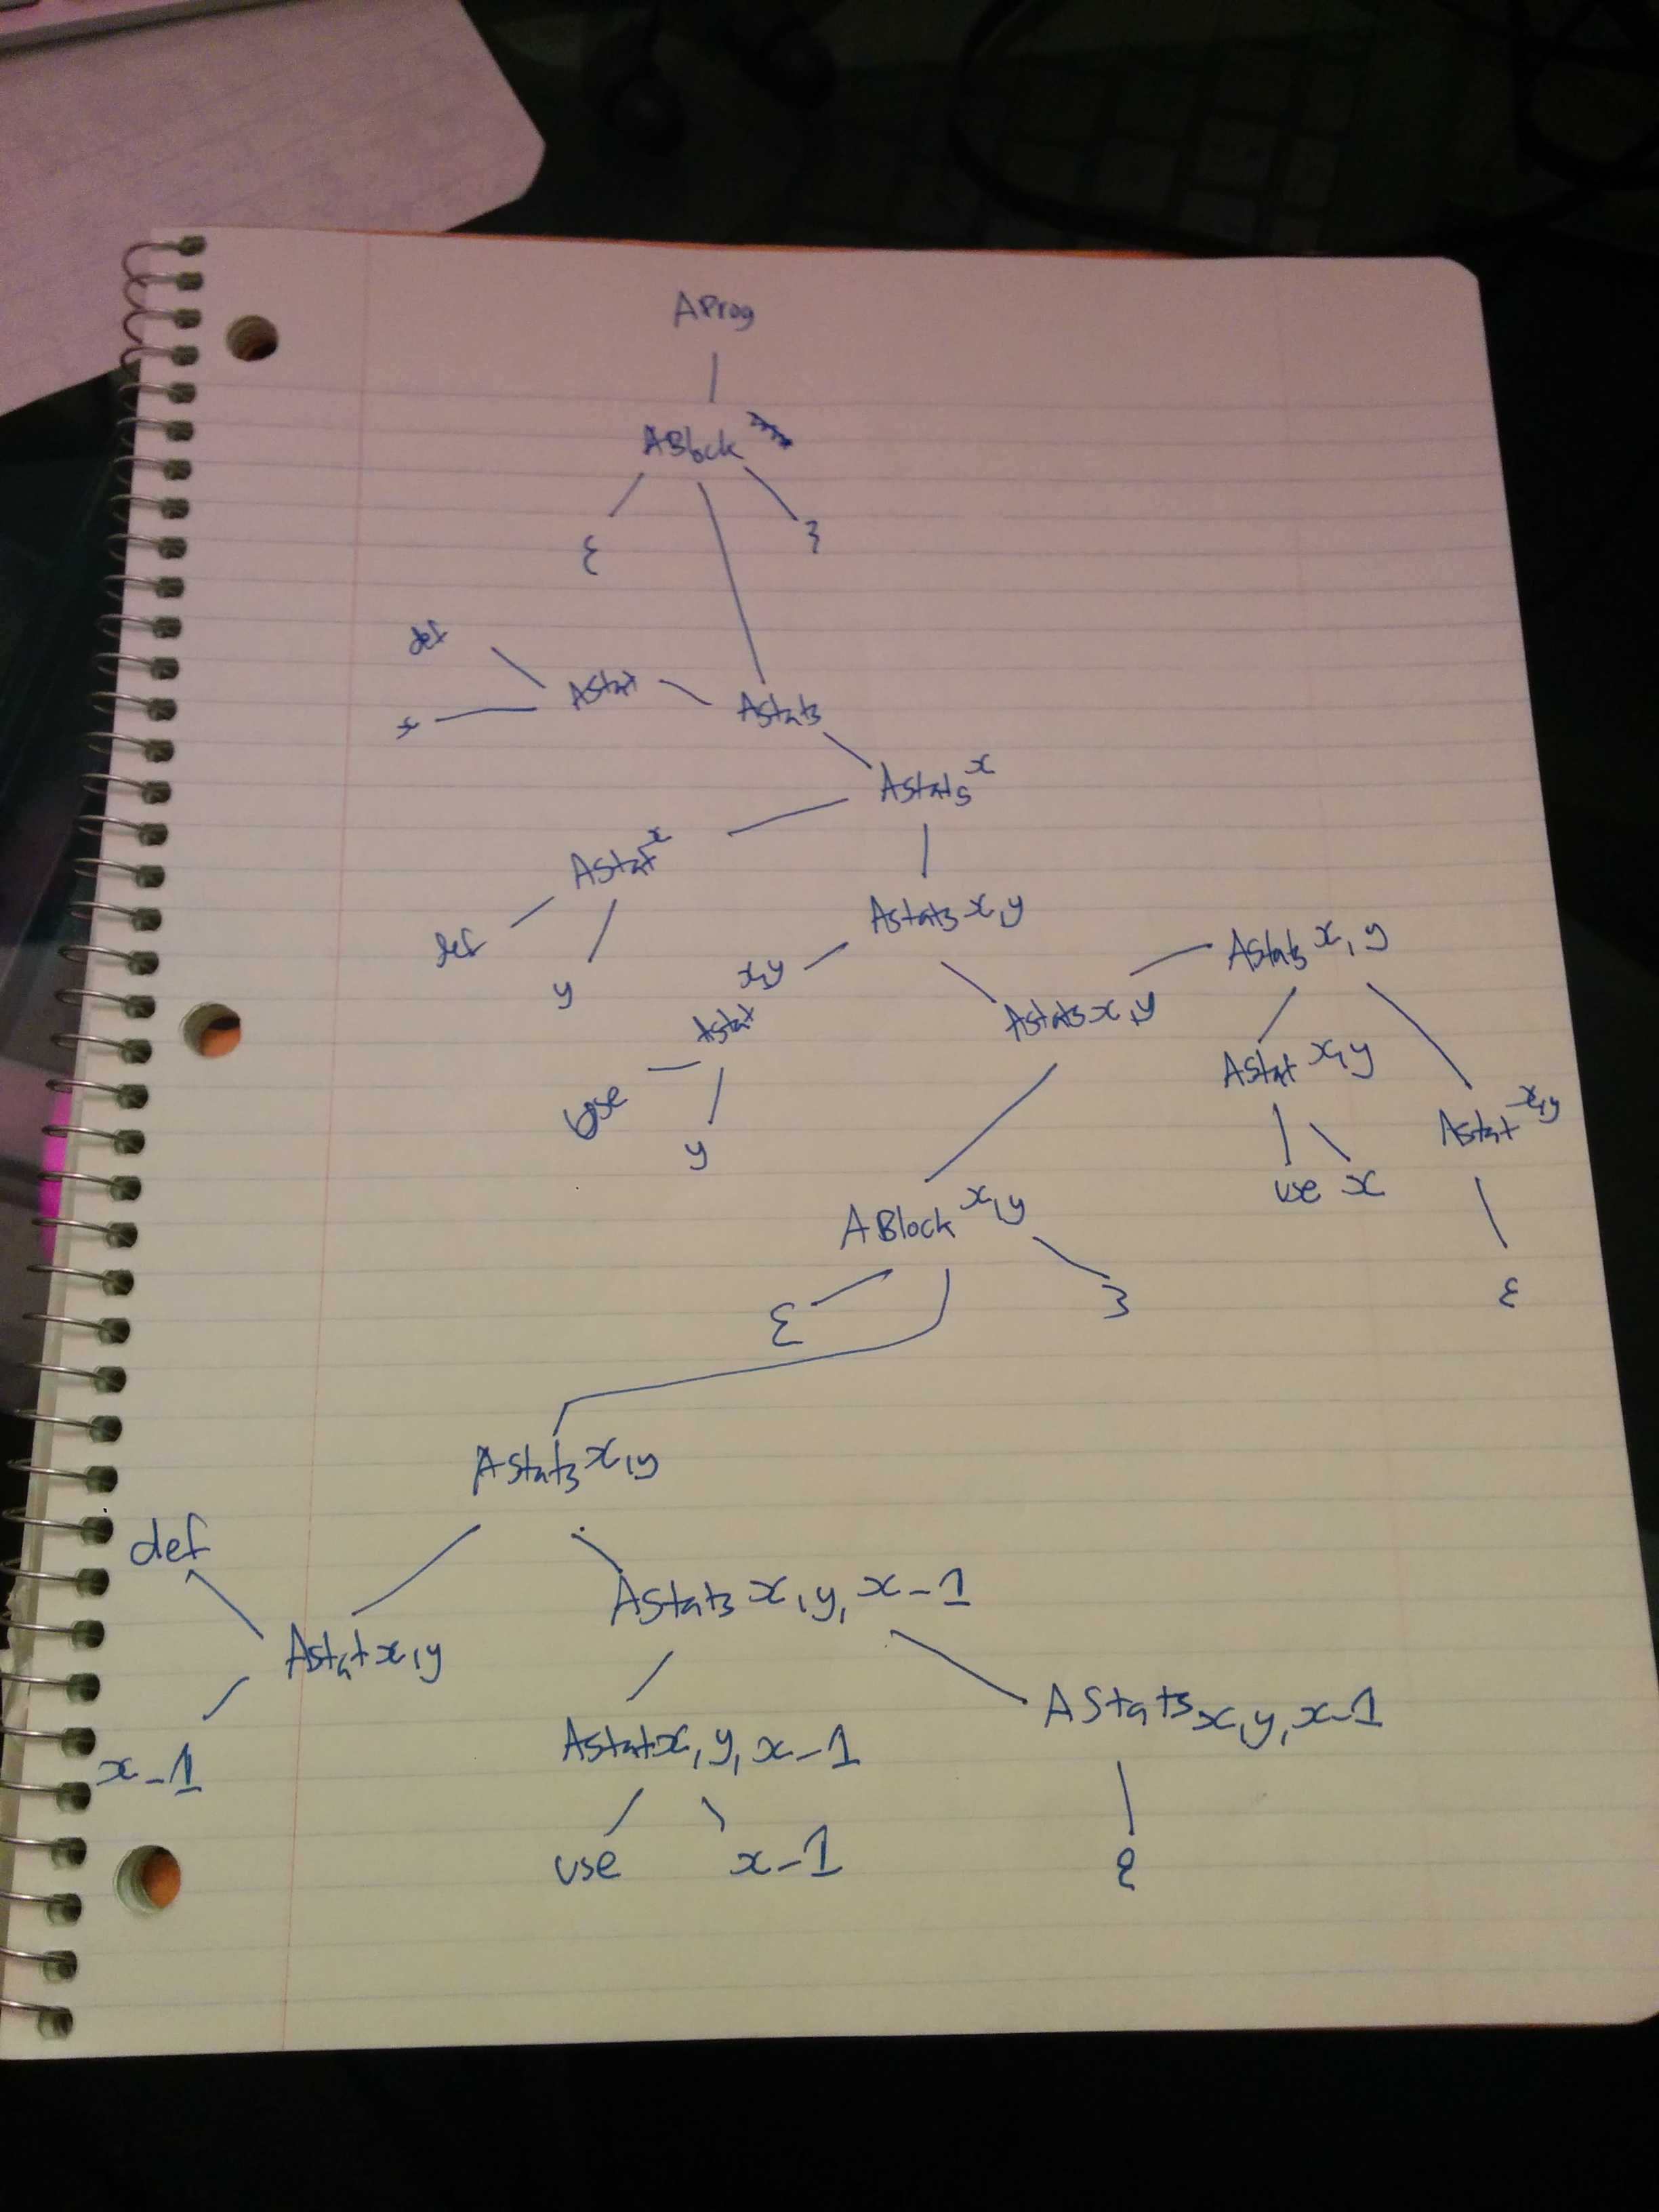
\includegraphics[scale=0.19]{IMG_20141008_212636.jpg}

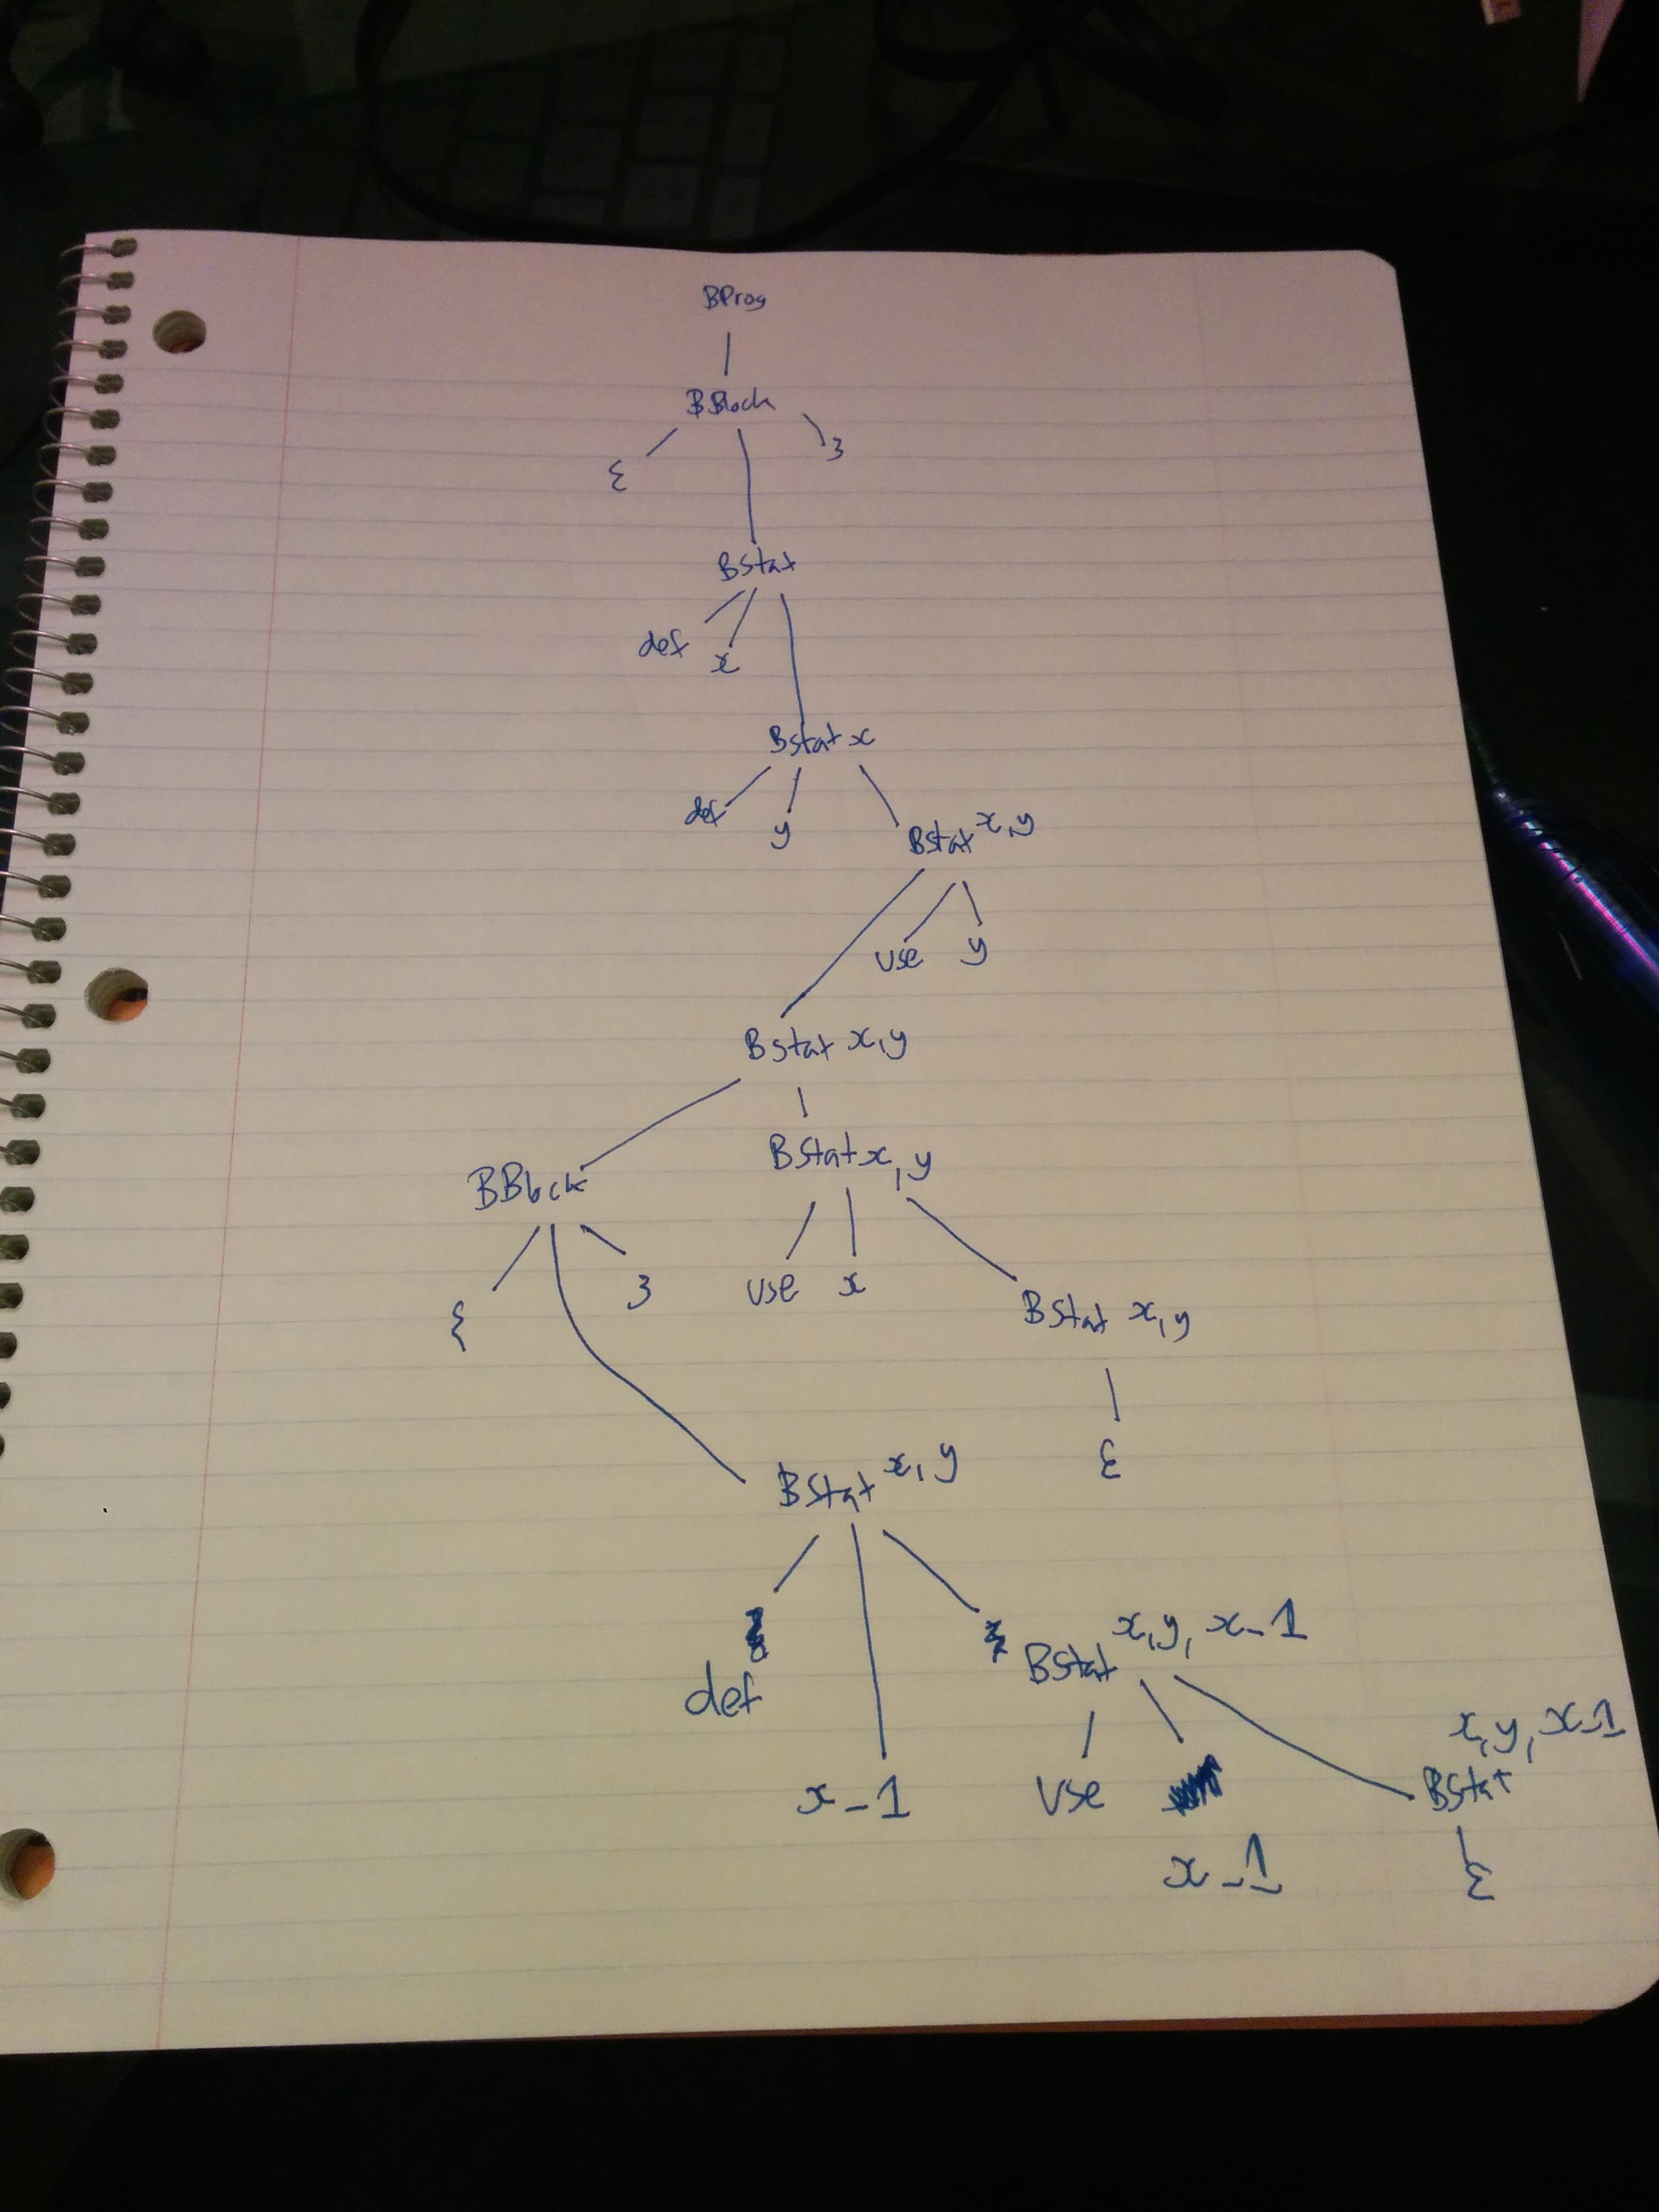
\includegraphics[scale=0.19]{IMG_20141008_212321.jpg}

\subsection{Question 1.2}

\par I didn't quite understand this, but my logic was to try and keep track of the variables and when that particular id was used I would assign yes. I could not just put everything into i, but I had to put it into ok so I used it as a store, as a yes, and as a false.

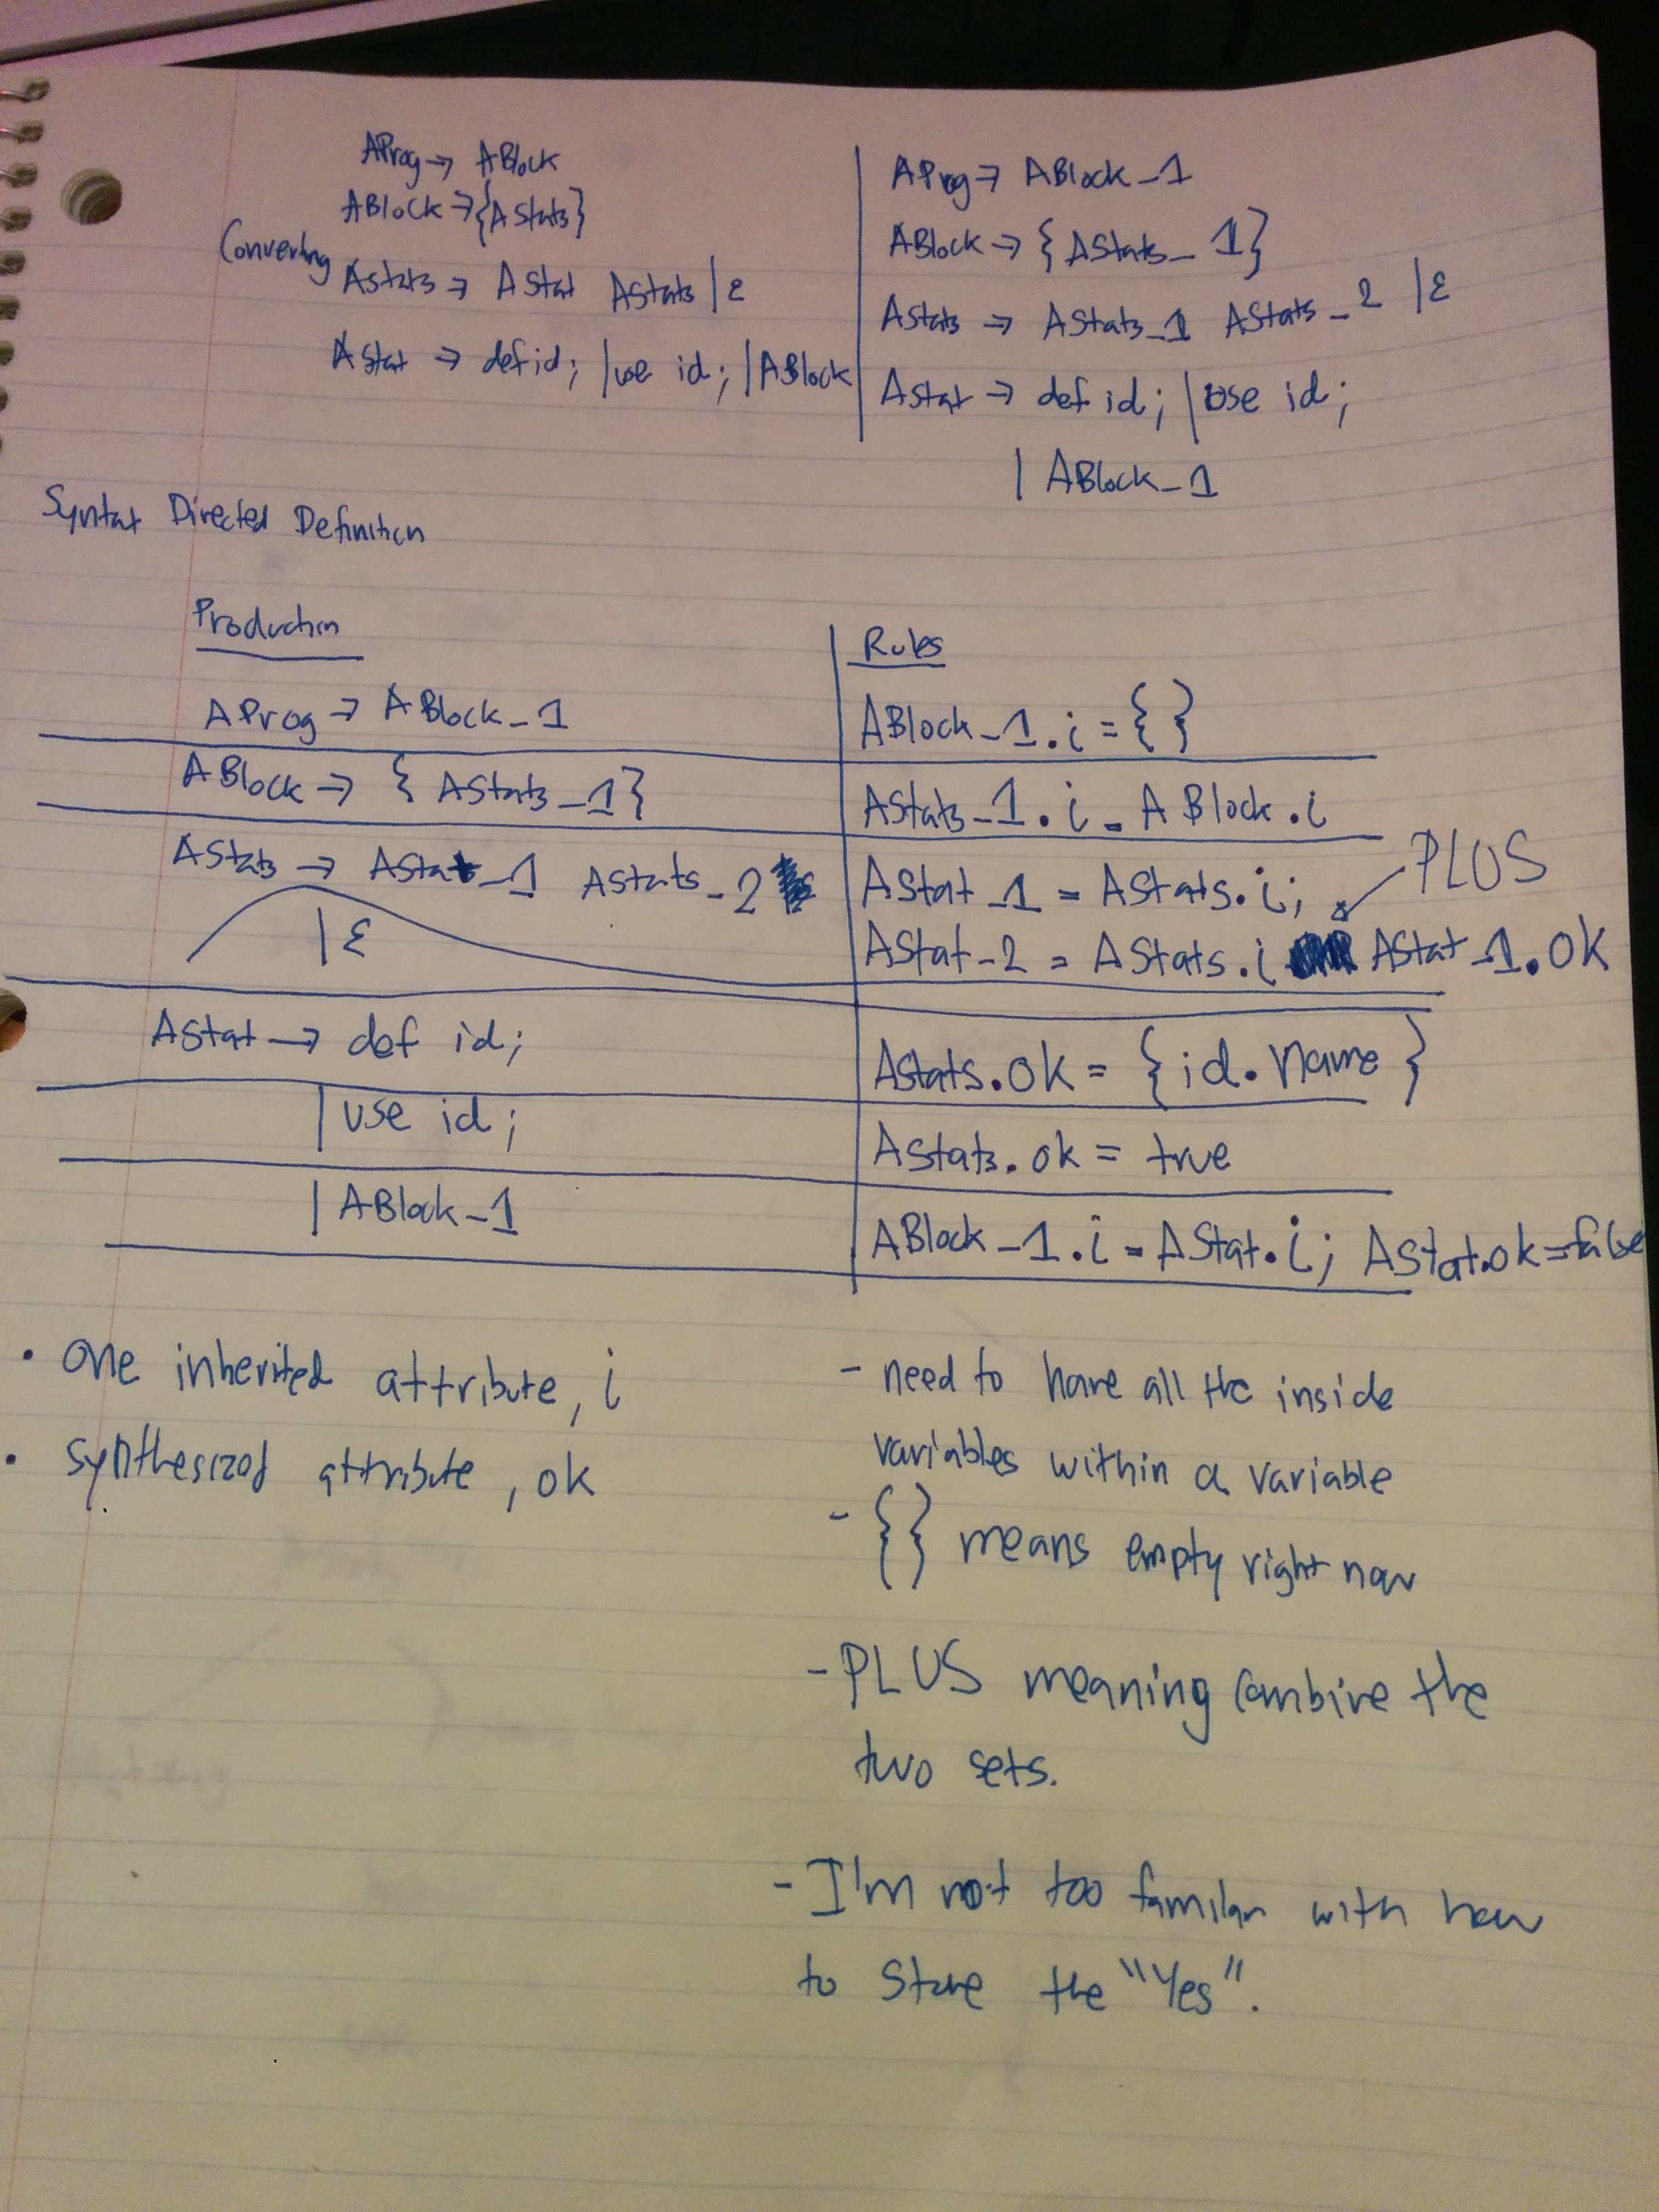
\includegraphics[scale=0.15]{IMG_20141008_215627.jpg}

\subsection{Question 1.3}

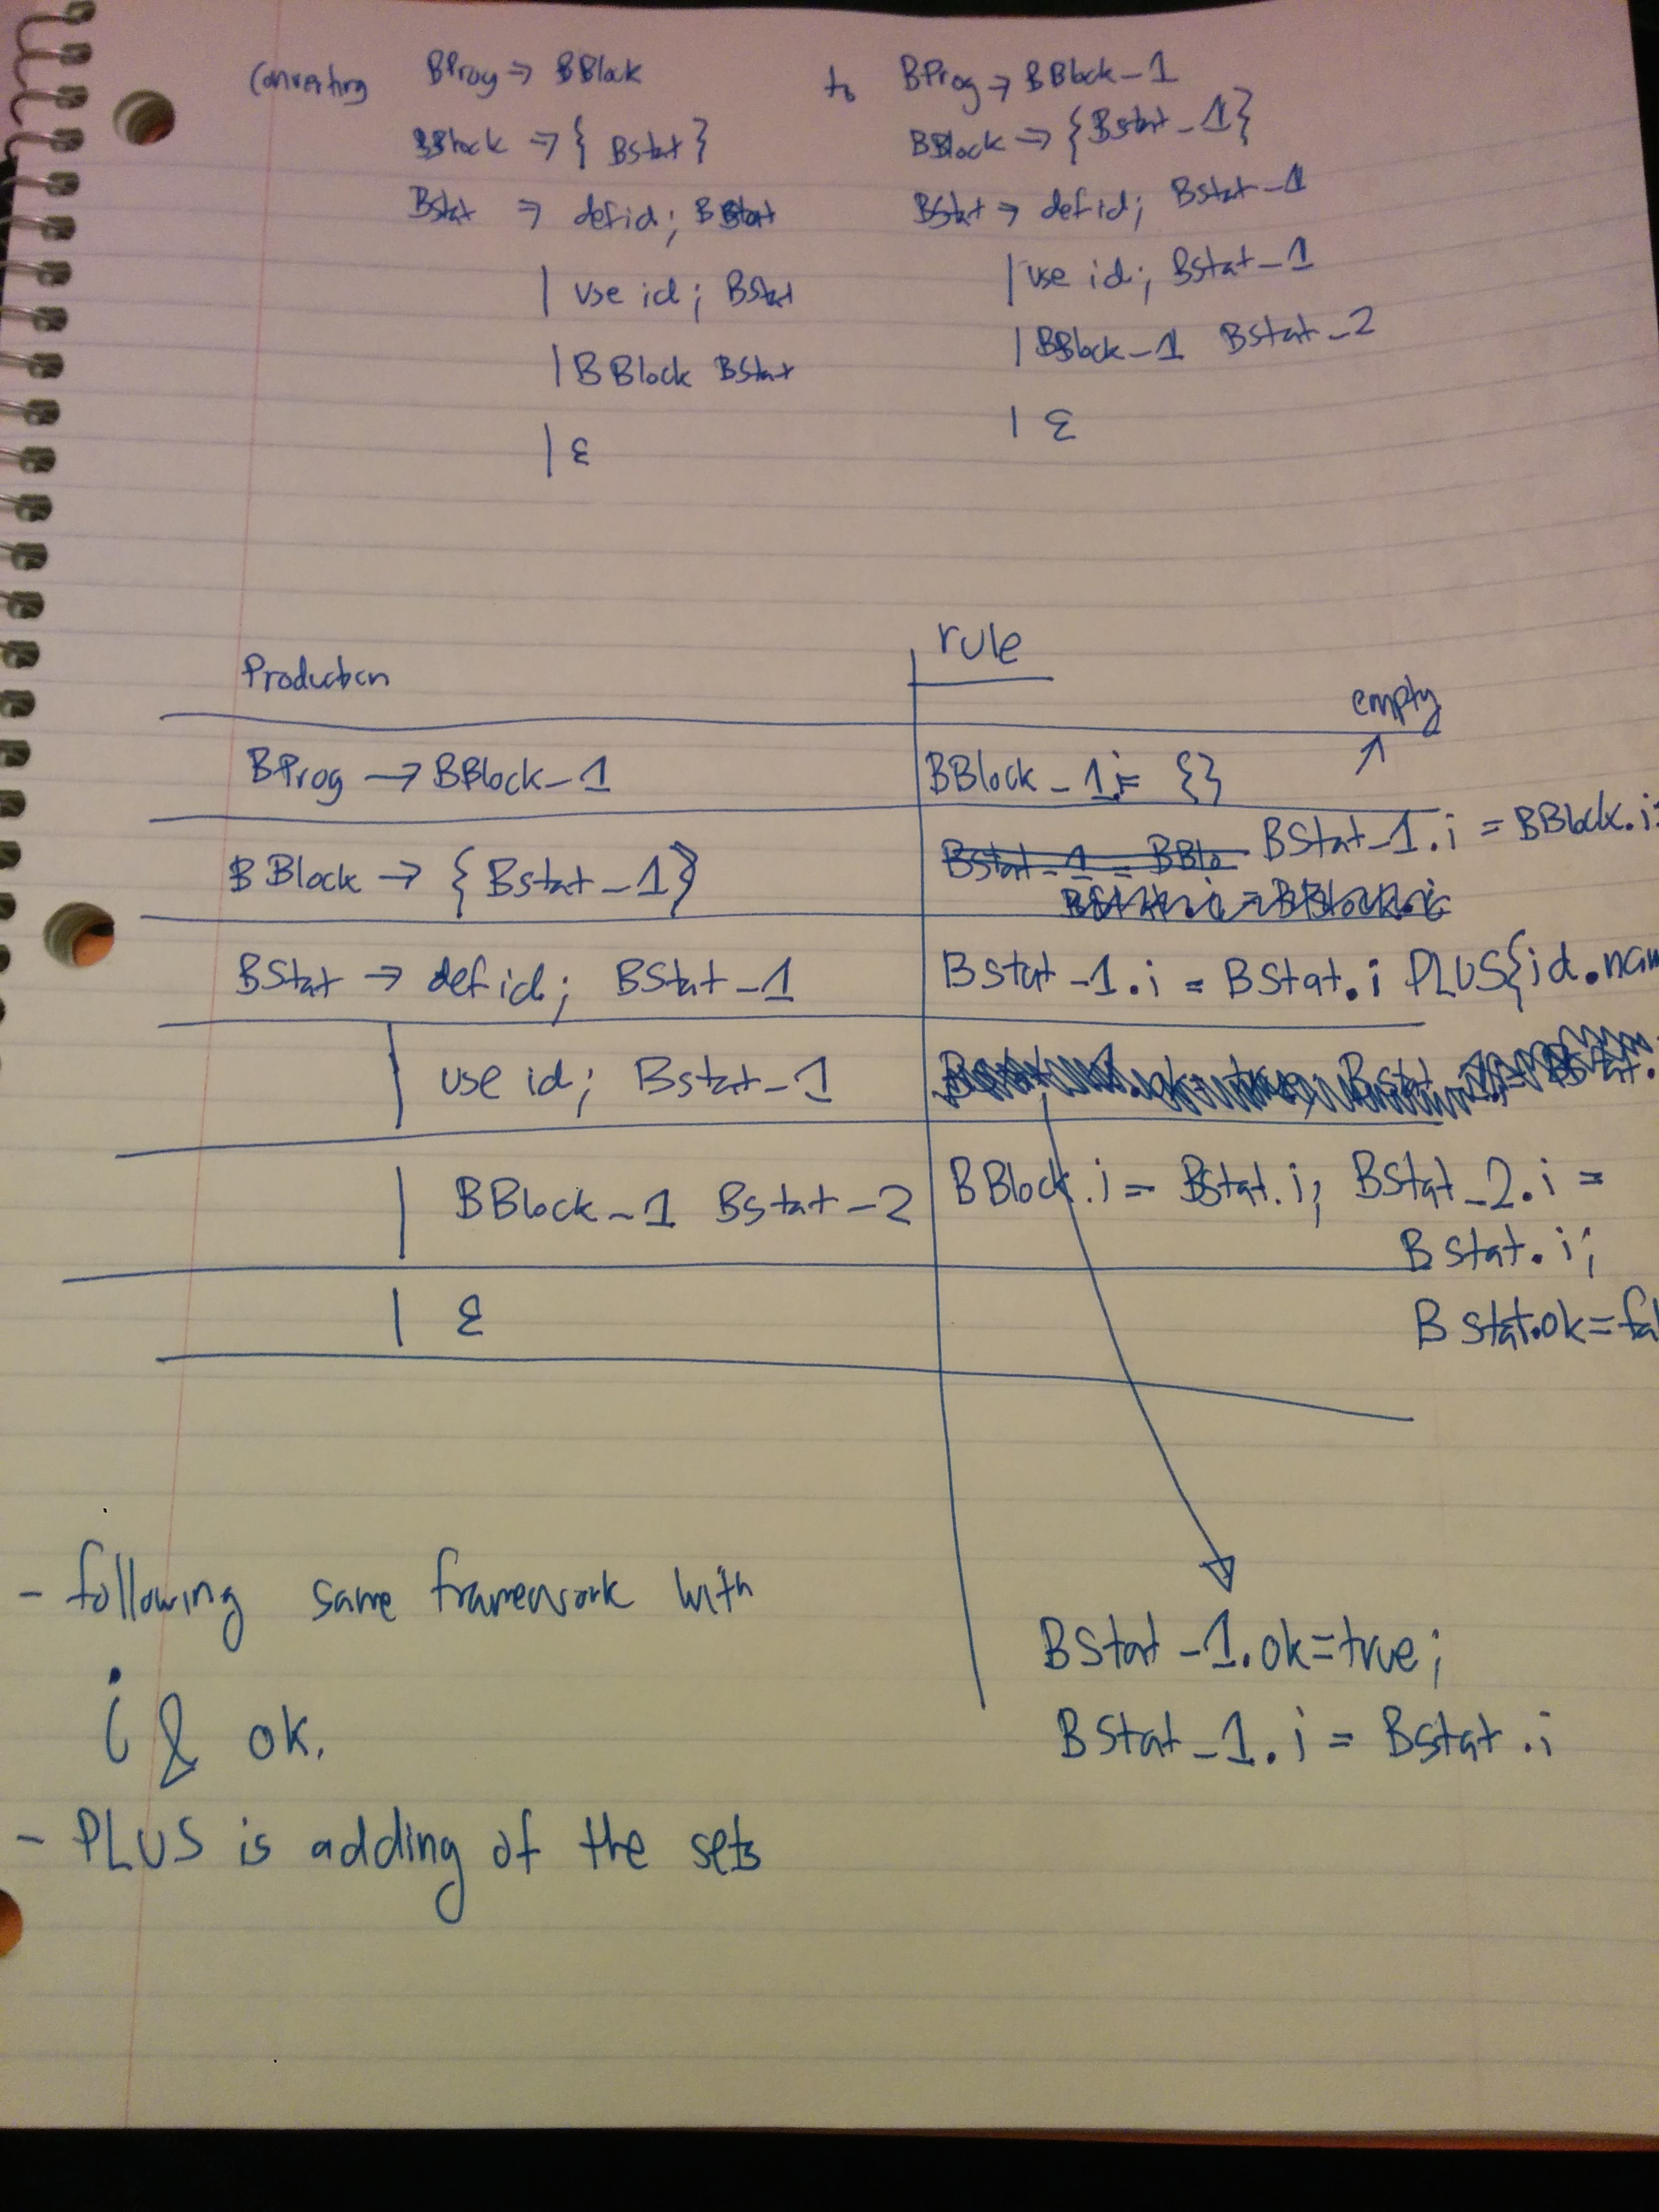
\includegraphics[scale=0.15]{IMG_20141008_222706.jpg}

\end{document} 